%\documentclass[12pt]{report}
%\usepackage[margin=2.5cm]{geometry}    % formatting 

\documentclass[english, 12pt, a4paper, online]{article} 
%\usepackage{a4wide}
\usepackage[margin=2cm]{geometry}
\usepackage{fancyhdr}                  % headers and footers
\usepackage{graphicx, placeins, subcaption, float, floatflt, wrapfig, placeins, adjustbox}         % Required for inserting images
\usepackage{amsmath,amsfonts,amssymb, bm, bbold} % math
\usepackage{siunitx}                   % typing values with units
\usepackage{biblatex}
\usepackage{tabto}                     % tabs on title page
\usepackage[colorlinks=true, allcolors=blue]{hyperref}  %blue links for titlepage :3
\usepackage{parskip} % paragraph changing
\usepackage[printonlyused, smaller]{acronym}
\usepackage{dsfont}

\usepackage{lipsum} % sample text
\usepackage{listings} % Including code into file
\usepackage{color}

\usepackage{cancel} % cancel out text

\usepackage{verbatim}   % comment blocks

\usepackage{pdfpages} % Include pdf pages 

\definecolor{mygreen}{rgb}{0,0.6,0}
\definecolor{mygray}{rgb}{0.5,0.5,0.5}
\definecolor{mymauve}{rgb}{0.58,0,0.82}

\lstset{ %
  backgroundcolor=\color{white},   % choose the background color
  basicstyle=\footnotesize,        % size of fonts used for the code
  breaklines=true,                 % automatic line breaking only at whitespace
  captionpos=b,                    % sets the caption-position to bottom
  commentstyle=\color{mygreen},    % comment style
  escapeinside={\%*}{*)},          % if you want to add LaTeX within your code
  keywordstyle=\color{blue},       % keyword style
  stringstyle=\color{mymauve},     % string literal style
}

\usepackage[toc,page]{appendix} % For appendices


% Setup for page numbering so far
\pagestyle{fancy}
\renewcommand{\headrulewidth}{0pt}
\fancyhead{}
\fancyfoot{} 
\fancyfoot[R]{\thepage}

\addbibresource{references.bib}

\setlength{\parindent}{0pt}

\newcommand{\TODO}[1]{\textcolor{red}{TODO: #1}}



\begin{document}


% Document chapters
\pagenumbering{roman}
\begin{titlepage}
    \begin{center}
    
        \vspace*{1cm}
        \Huge
        \textbf{
        Combined Report for all Practicals}
            
        \vspace{0.5cm}
        \LARGE
        M32 Signal and image processing

            
        \vspace{2cm}
        \Large
        \begin{flushleft}
            \text{Benjamin AKERLUND}    \tab\url{benker-3@student.ltu.se} \\
            \text{Louis BARBOUTIE}      \tab\url{loubar-3@student.ltu.se}     
            
        \end{flushleft}
            
        \vfill
            
        %\includegraphics[width=0.4\textwidth]{Graphics/LTU_logo.png}
        
\includegraphics[width=0.5\linewidth]{Graphics/Vignette logo.png}
        \vfill
   
        
        \begin{flushleft}
            \large
            M2 - \ac{TSI}\\
            Faculty of Science and Engineering (\textit{Faculté sciences et ingénierie}) \\
            \ac{UPS} \\
            \today
        \end{flushleft}
                   
            
    \end{center}
\end{titlepage}
\addcontentsline{toc}{section}{Preface}
\section*{Preface}


This report is a submission for the \textit{M32 Signal and Image Processing} course at \ac{UPS} during the autumn semester of 2024.
This submissionn contains all practical assignments given in the three parts of the graded assignments for this course, i.e., \textit{BE1\_IntroComputerVision}, \textit{BE2\_IntroMorphoMath} and \textit{BE3\_ShapeDetection}.

This report is a joint effort of the students mentioned on the title page and is submitted as a group project, as instructed by the lecturer.
The full list of project files can be found in the following GitHub repository: \url{https://github.com/benjaminakerlund/ut3-Image_Processing}.

This submission contains the following source files:
\begin{itemize}
    \item report.pdf, this report
    \item part1.m, source code for part 1
    \item part2.m, source code for part 2
    \item part3.m, source code for part 3
\end{itemize}




% Move later to own page in main.tex if does not fit well here
\vspace{2cm}
%% Created: Vincent Brückner
%% define acronym, eg. LTU:              \acro{LTU}{Luleå University of Technology}
%% use in text:                 \ac{LTU} -> first time: Luleå University of Technology (LTU) ;-> all following times: LTU
%% (Note capital letters)
%% force long version in text:  \acf{LTU} -> Luleå University of Technology (LTU)
%% force short version in text: \acs{LTU} -> LTU
%% long version without LTU:    \acl{LTU} -> Luleå University of Technology
%% More info: https://ftp.acc.umu.se/mirror/CTAN/macros/latex/contrib/acronym/acronym.pdf

%% Before publishing: Copy all acronyms into Excel and sort by alphabetic order


\addcontentsline{toc}{section}{Symbols and Abbreviations}
\section*{Symbols and Abbreviations}


\subsection*{Abbreviations}
\label{subsec:abbreviations}

\begin{acronym}[CCSDSCC] % [longest acronym]
    \acro{ASEP}{LEO PLS FILL IN HERE...}
    \acro{LTU}{Luleå University of Technology}
    \acro{ML}{Maximum Likelihood estimator}
    \acro{PSF}{Point Spread Function}
    \acro{TSI}{Space Technology and Instrumentation}
    \acro{UPS}{Université Toulouse III - Paul Sabatier}
\end{acronym}






%\addcontentsline{toc}{section}{Abstract}
\section*{Abstract}



\begin{table}[h]
    \begin{tabular}{|p{\linewidth}|}
        \hline \\
        Using \ac{SPENVIS}, this report investigates the spacecraft environment for a specific pre-determined orbit corresponding to a so-called Molniya orbit.
        This report analyses the expected spacecraft environment and gives recommendations on design choices: specifically the thickness of solar panel cover glass, the thickness of aluminium shielding for memory devices and the selection of one Integrated Circuit chip over another. 
        \\~\\
        \textit{"\acs{SPENVIS} is \ac{ESA}'s \acf{SPENVIS}, a WWW interface to models of the space environment and its effects; including galactic cosmic rays, solar energetic particles, natural radiation belts, plasmas, gases, meteoroids and debris."} \cite{spenvis_webpage}.
        \\
        \hline
    \end{tabular}
    \label{abbreviations}
\end{table}
\textbf{Keywords:} SPENVIS, ESA, Spacecraft Environment, Space Environment, Single Event Effect, Single Event Upset, CMOS, Solar degradation, 

\vspace{2cm}
        \begin{figure}[h]
            \centering
            \includegraphics[width=0.3\textwidth]{Graphics/spenvislogo.png}
            \hspace{1cm}\includegraphics[width=0.3\textwidth]{Graphics/esa.png}
        \end{figure}
%%% Created: Vincent Brückner
%% define acronym, eg. LTU:              \acro{LTU}{Luleå University of Technology}
%% use in text:                 \ac{LTU} -> first time: Luleå University of Technology (LTU) ;-> all following times: LTU
%% (Note capital letters)
%% force long version in text:  \acf{LTU} -> Luleå University of Technology (LTU)
%% force short version in text: \acs{LTU} -> LTU
%% long version without LTU:    \acl{LTU} -> Luleå University of Technology
%% More info: https://ftp.acc.umu.se/mirror/CTAN/macros/latex/contrib/acronym/acronym.pdf

%% Before publishing: Copy all acronyms into Excel and sort by alphabetic order


\addcontentsline{toc}{section}{Symbols and Abbreviations}
\section*{Symbols and Abbreviations}


\subsection*{Abbreviations}
\label{subsec:abbreviations}

\begin{acronym}[CCSDSCC] % [longest acronym]
    \acro{ASEP}{LEO PLS FILL IN HERE...}
    \acro{LTU}{Luleå University of Technology}
    \acro{ML}{Maximum Likelihood estimator}
    \acro{PSF}{Point Spread Function}
    \acro{TSI}{Space Technology and Instrumentation}
    \acro{UPS}{Université Toulouse III - Paul Sabatier}
\end{acronym}

\tableofcontents
\addcontentsline{toc}{section}{Contents}
\include{} % DO NOT REMOVE

% content chapters
\pagenumbering{arabic}
\include{Text/0}
\section{Introduction to Computer vision}
\label{sec:introduction_to_computer_vision}

Exercises for \textit{BE1\_IntroComputerVision} practical.

\subsection{Basics}

\textbf{Question 1:}
\textit{Load and Display a grayscale image and a color image. How do you interpret the image coding under MatLab? What is the data type?}

\begin{figure}[H]
    \centering
    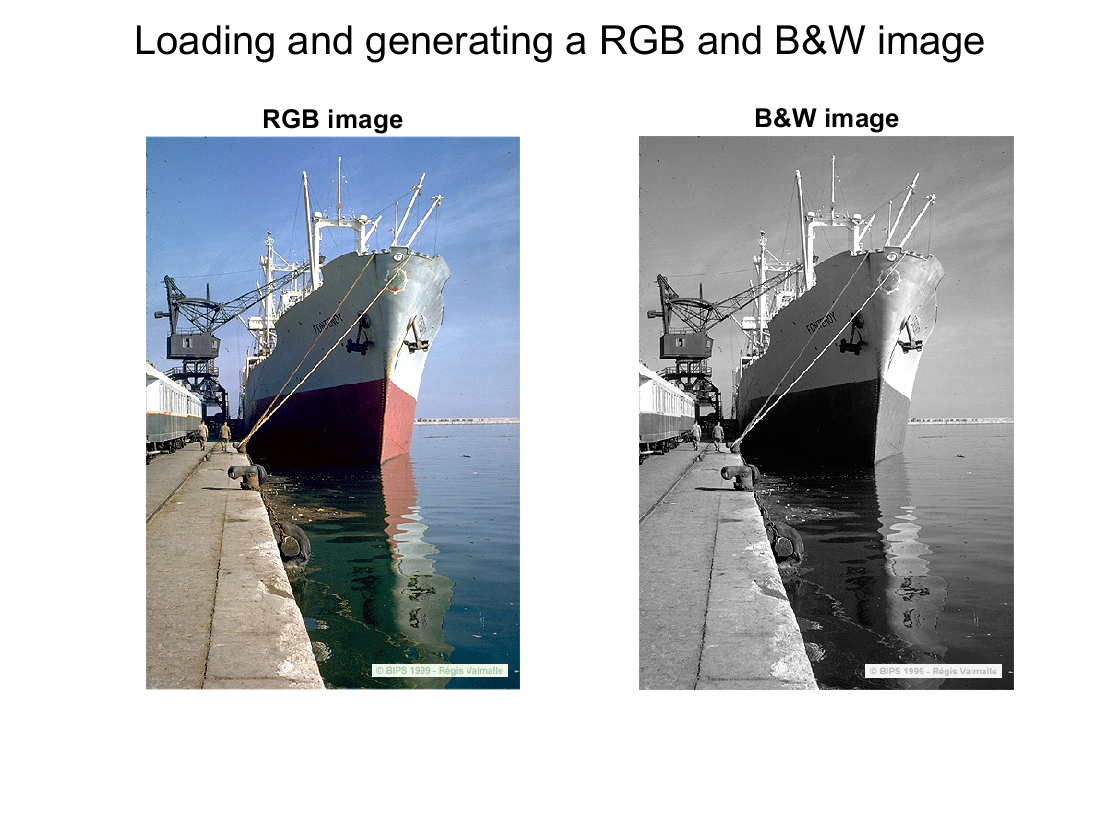
\includegraphics[width=0.5\linewidth]{Doc/Graphics/Part1_Question1.png}
    \label{fig:enter-label}
\end{figure}


\subsubsection{Greyscale Image Coding}

\textbf{Question 2:}
\textit{Build a matrix with a gradual value of intensity and an horizontal line with a constant value; the representative image is shown Fig. 1.}

\begin{figure}[H]
    \centering
    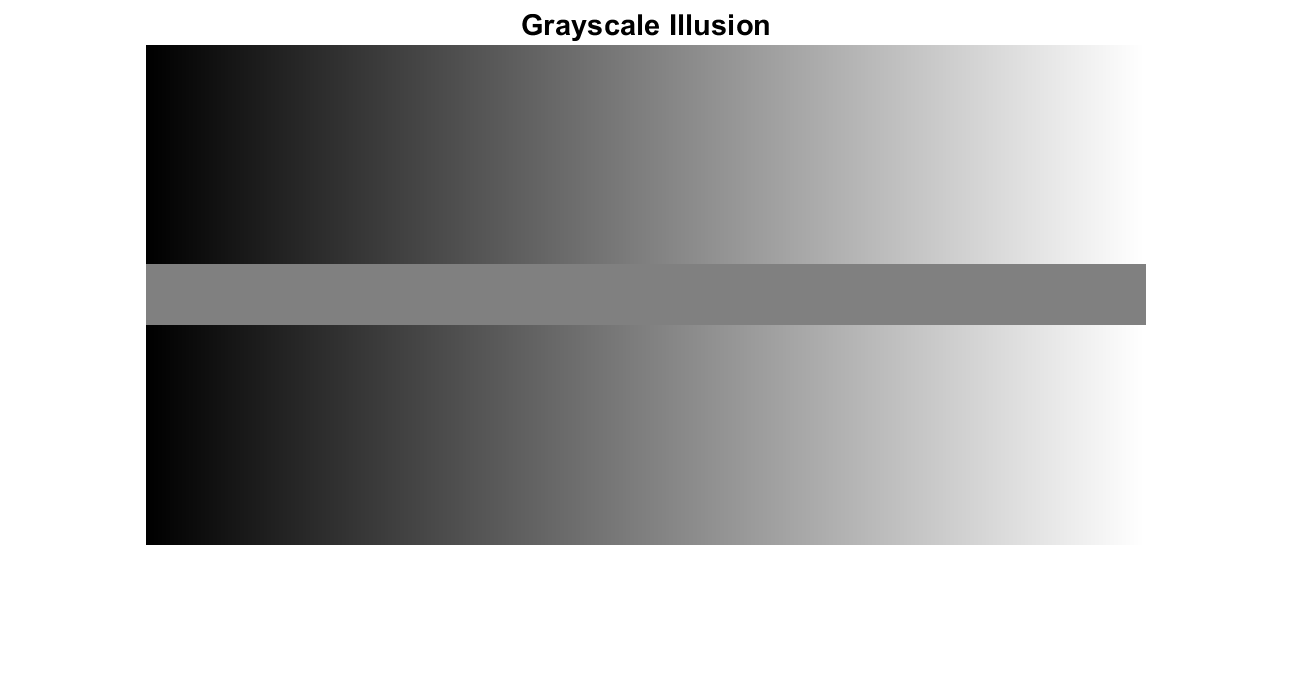
\includegraphics[width=0.5\linewidth]{Doc/Graphics/Part1_Question2.png}
    \label{fig:enter-label}
\end{figure}



\textbf{Question 3:}
\textit{Build a matrix of black \& white stripes, and with a rectangle and disk as shown Fig. 2. All parameters (size of stripes, size of rectangle, radius) should be easily modifiable.}

\begin{figure}[H]
    \centering
    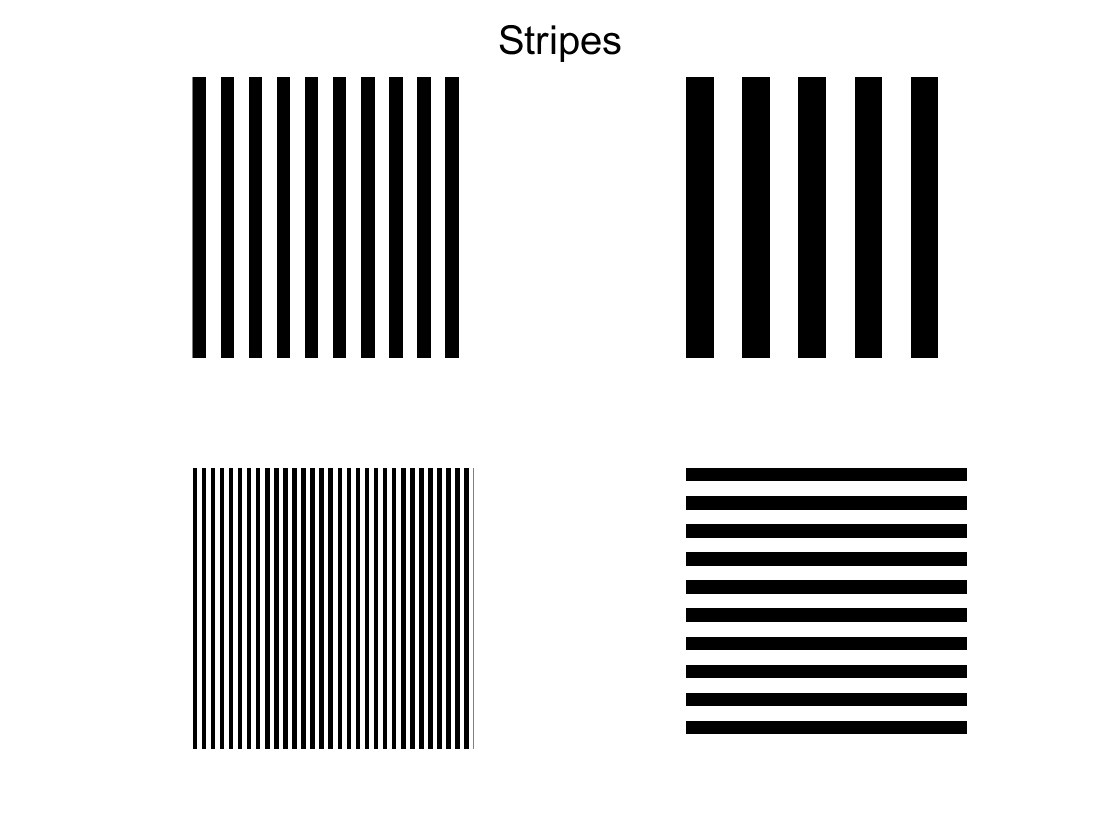
\includegraphics[width=0.75\linewidth]{Doc/Graphics/Part1_Question3a.png}
    \label{fig:enter-label}
\end{figure}

\begin{figure}[H]
    \centering
    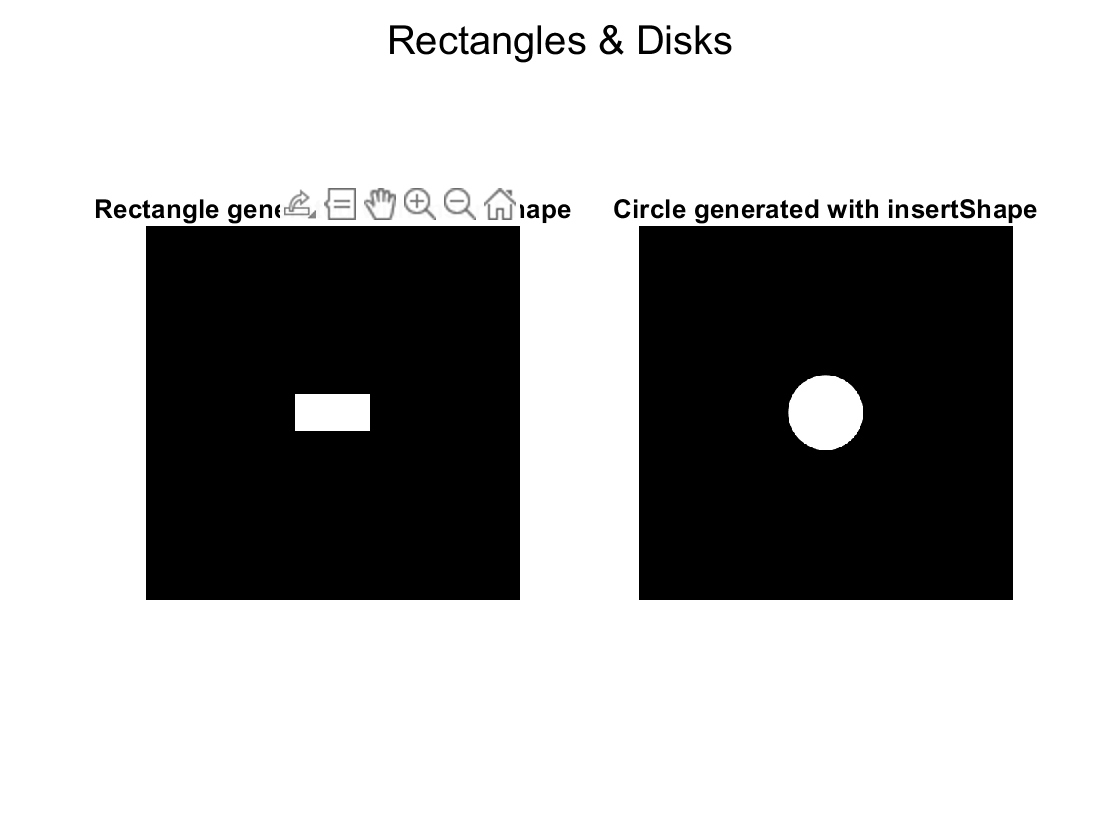
\includegraphics[width=0.5\linewidth]{Doc/Graphics/Part1_Question3b.png}
    \label{fig:enter-label}
\end{figure}



\subsubsection{Colour Image Coding}
\textbf{Question 4:}
\textit{Next, display Teinte.jpg and its red, green and blue components. Interpret and analyse. Same with oeil.jpg, cargo.jpg and CoulAdd.jpg.}

\begin{figure}[H]
    \centering
    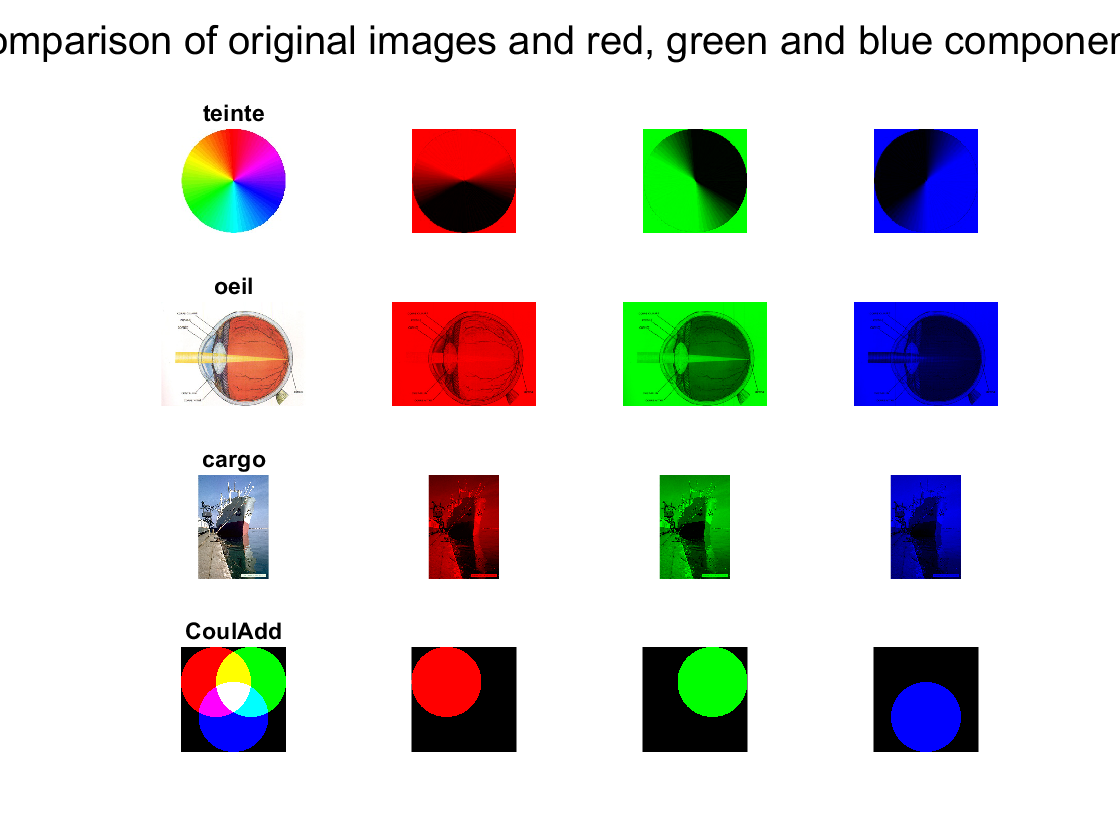
\includegraphics[width=\linewidth]{Doc/Graphics/Part1_Question4a.png}
    \label{fig:enter-label}
\end{figure}



\textbf{Question 5:}
\textit{Build and display the french flag. Build and display your flag.}

\begin{figure}[H]
    \centering
    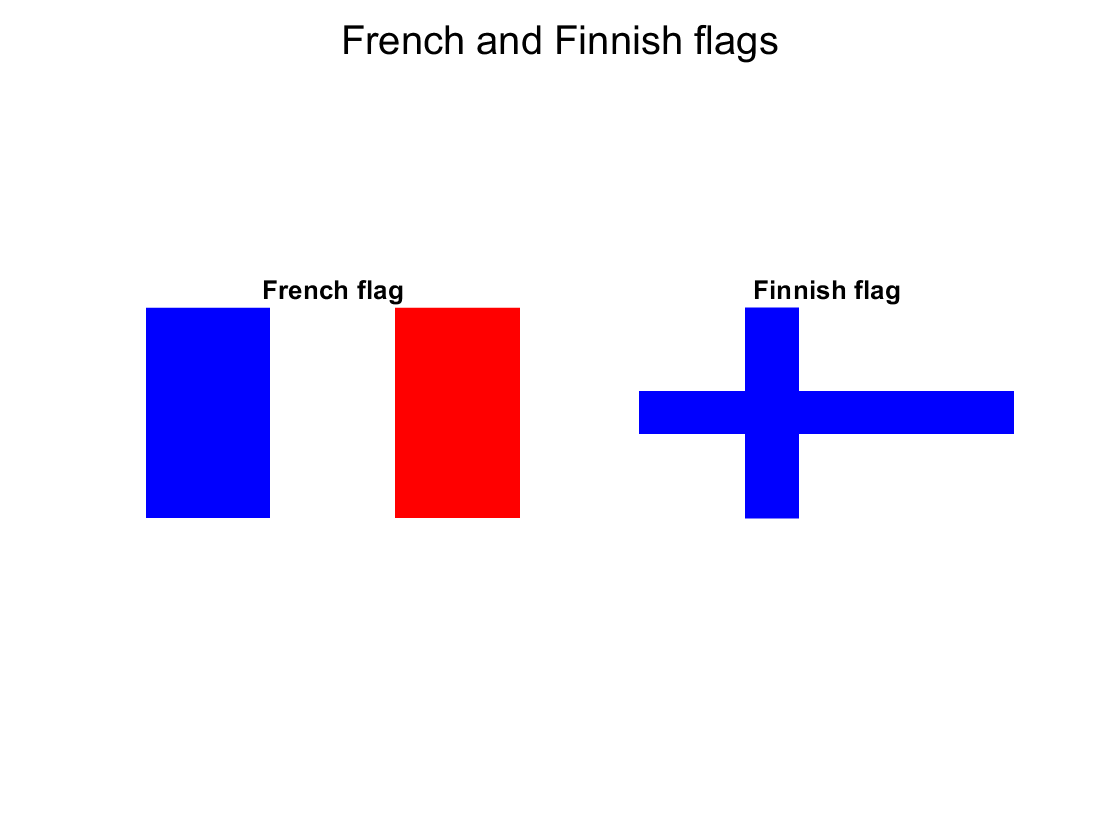
\includegraphics[width=0.5\linewidth]{Doc/Graphics/Part1_Question5.png}
    \label{fig:enter-label}
\end{figure}



\textbf{Question 6:}
\textit{Use the HSV code (with the command rgb2hsv and interpret images. How is the type of the new matrix? Build and display the image Fig. 4.}

\begin{figure}[H]
    \centering
    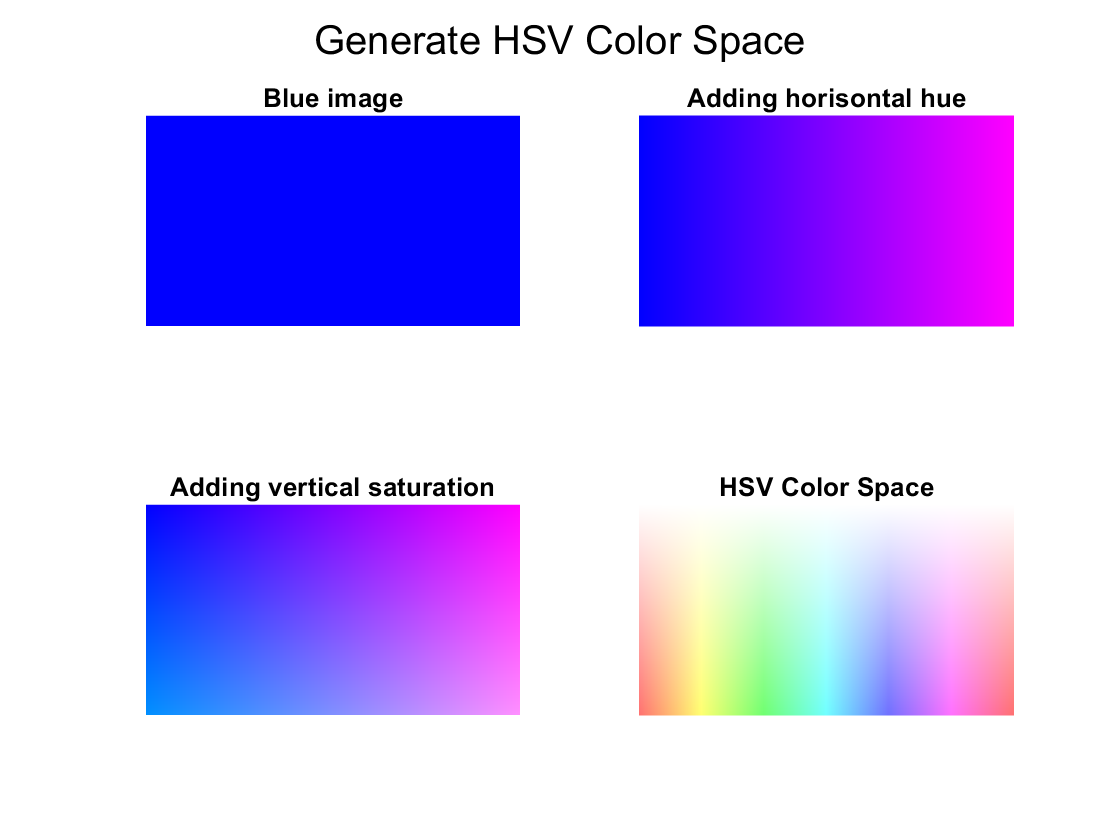
\includegraphics[width=0.75\linewidth]{Doc/Graphics/Part1_Question6a.png}
    \label{fig:enter-label}
\end{figure}

\begin{figure}[H]
    \centering
    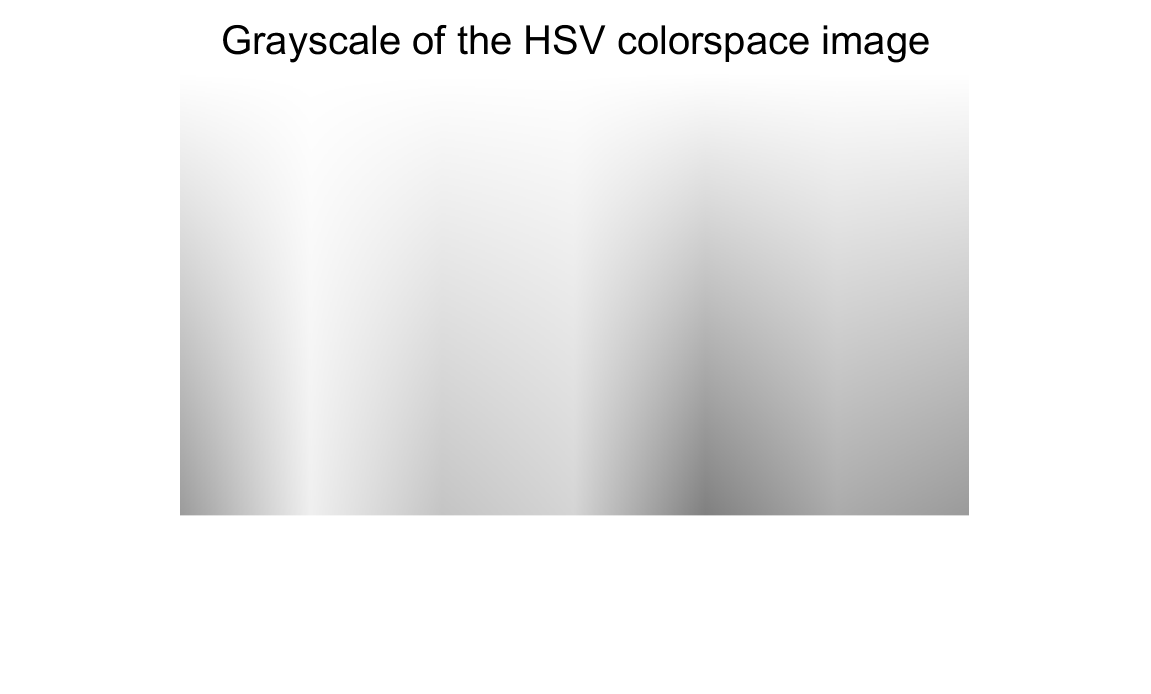
\includegraphics[width=0.5\linewidth]{Doc/Graphics/Part1_Question6b.png}
    \label{fig:enter-label}
\end{figure}



\textbf{Question 7:}
\textit{What are the values of $\alpha$, $\beta$ and $\gamma$?}

\TODO{}



\textbf{Question 8:}
\textit{Load and display SpainBeach.png and isolate the beach.}

\TODO{Any commentary on how we did this?}

\begin{figure}[H]
    \centering
    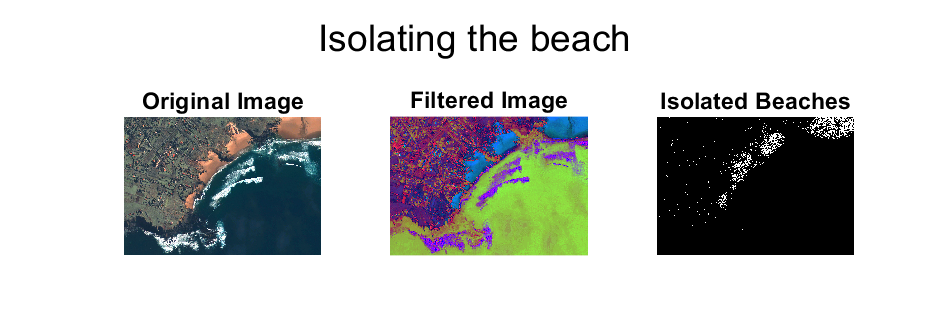
\includegraphics[width=\linewidth]{Doc/Graphics/Part1_Question8.png}
    \label{fig:enter-label}
\end{figure}



\subsubsection{Histograms}
\textbf{Question 9:}
\textit{What is a histogram? What is the use? Display and interpret histograms of images.}

A histogram of an image represents the intensity level repartition in the image according to the following equation:
\[H_I(n) = \sum_{u} \sum_{v} \{ I(u, v) = n \}\]

However, spatial information is lost. 
If we take the histogram of the Grayscale illusion we can see that the color value in the center bar is clearly overrepresented.

\TODO{INSERT FIGURE}



\textbf{Question 10:}
\textit{Work the mysterious images called Imagex.bmp and Imagexx.bmp.}

\TODO{What the hell does "work the images" mean? XDD}





\subsubsection{Filtering}
\textbf{Question 11:}
\textit{Apply blur Filtering and Edge filtering on the Stripes images and on a ’real’ image. What are the main associated Kernels ?}



\textbf{Question 12:}
\textit{Thanks to successive filtering operators, isolate the main 5 stars of the image Etoile.png.}


\subsection{Fourier Transform}
\textbf{Question 13:}
\textit{Get the FT and analyze the spectrum if images with stripes (Fig. 2), rectangle and disks (Fig. 3).}



\textbf{Question 14:}
\textit{Blur the image with different kernels and interpret the spectrum.}



\textbf{Question 15:}
\textit{Write a program that extracts the specific field in the image Champs.jpg (see Fig. 5).}
\begin{figure}[H]
    \centering
    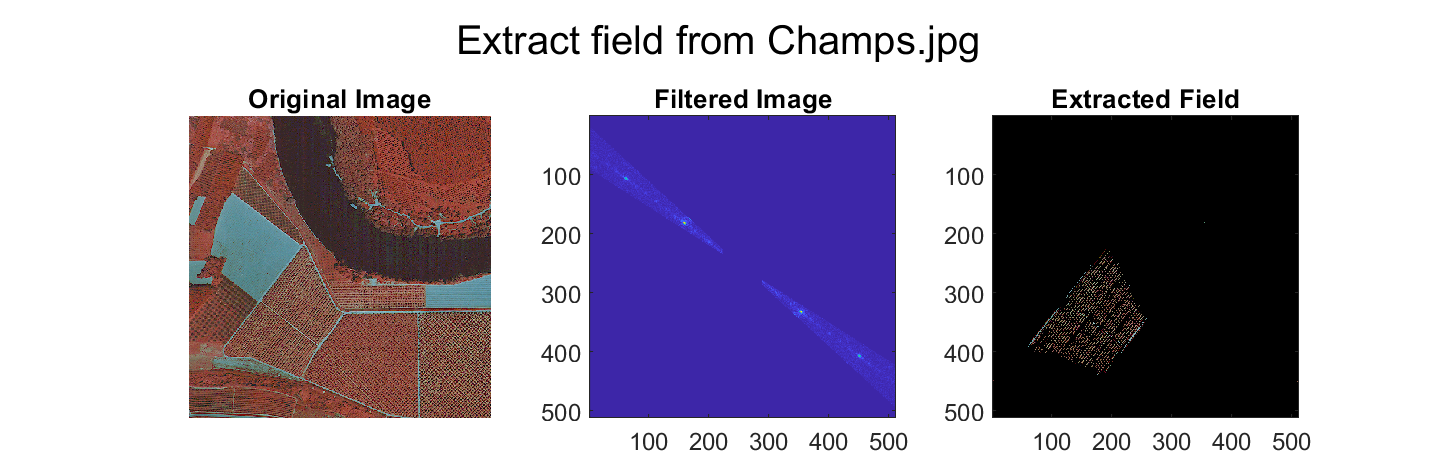
\includegraphics[width=\linewidth]{Doc/Graphics/Part1_Question15.png}
    \label{fig:enter-label}
\end{figure}


% ~~~~~~~~~~~~~~~~~~~~~~~~~~~~~~~~
% Subsection: Deblurring
% ~~~~~~~~~~~~~~~~~~~~~~~~~~~~~~~~
\subsection{Deblurring}
\subsubsection{Linear Modelization}
\textbf{Question 16:}
\textit{Why do we have chosen this model? What are the limits of this model with respect to a single lens model?}



\textbf{Question 17:}
\textit{Compare the spectrums of the original image and of the blur image: what do you observe? Justify.}



\subsubsection{Blur Estimation}
\textbf{Question 18:}
\textit{Propose a cardinal sinus function that have the same zeros than H(u) (superpose the two functions). What conclusion could you give from these properties? Could you estimate T ?}


\textbf{Question 19:}
\textit{Estimate T.}




\subsubsection{Image Deblurring}

The following program allows to apply this process (Inverse Filtering -> Wiener Filtering):
\begin{lstlisting}
    SeuilMax = 11 ;
    hh = zeros(TailleImage);
    centre = [1 1] + floor(TailleImage/2) ;
    ext = (TailleFiltre-[1 1])/2;
    ligs = centre(1) + [-ext(1):ext(1)];
    cols = centre(2) + [-ext(2):ext(2)];
    
    h = ones(TailleFiltre)/prod(TailleFiltre);
    hh(ligs,cols) = h;
    hh = ifftshift(hh);
    
    H = fft2(hh);
    
    ind = find(abs(H)<(1/SeuilMax));
    H(ind) = (1/SeuilMax)*exp(j*angle(H(ind)));
    
    G = ones(size(H))./H;
    
    (...)
\end{lstlisting}


\textbf{Question 20:}
\textit{Complete this program (only 2 lines!) to process inverse filtering method.}



\textbf{Question 21:}
\textit{What’s happen with the image marcheur.jpg ?}
\section{Introduction to Mathematical Morphology}
\label{sec:introduction_to_mathematical_morphology}



\setcounter{subsection}{1}
\subsection{Erosion and Dilation}
% question 2 image:
\textbf{Question 1} \textit{Define erosion and dilatation from an ensemblist point of view and an functional point of view. Give some properties related to these operators.}



\textbf{Question 2} \textit{Operate in a binary image and a greyscale image with the MatLab commands imerode and imdilate. What are the effects on binary and grayscale images? Justify. Try with different structuring elements (different shapes, different sizes).}

In the figure below, the eroded and dilated images can be seen plotted next to the original image for each structuring element with the following shapes in order: rectangle, disk, diamond and line.

\begin{figure}[H]
    \centering
    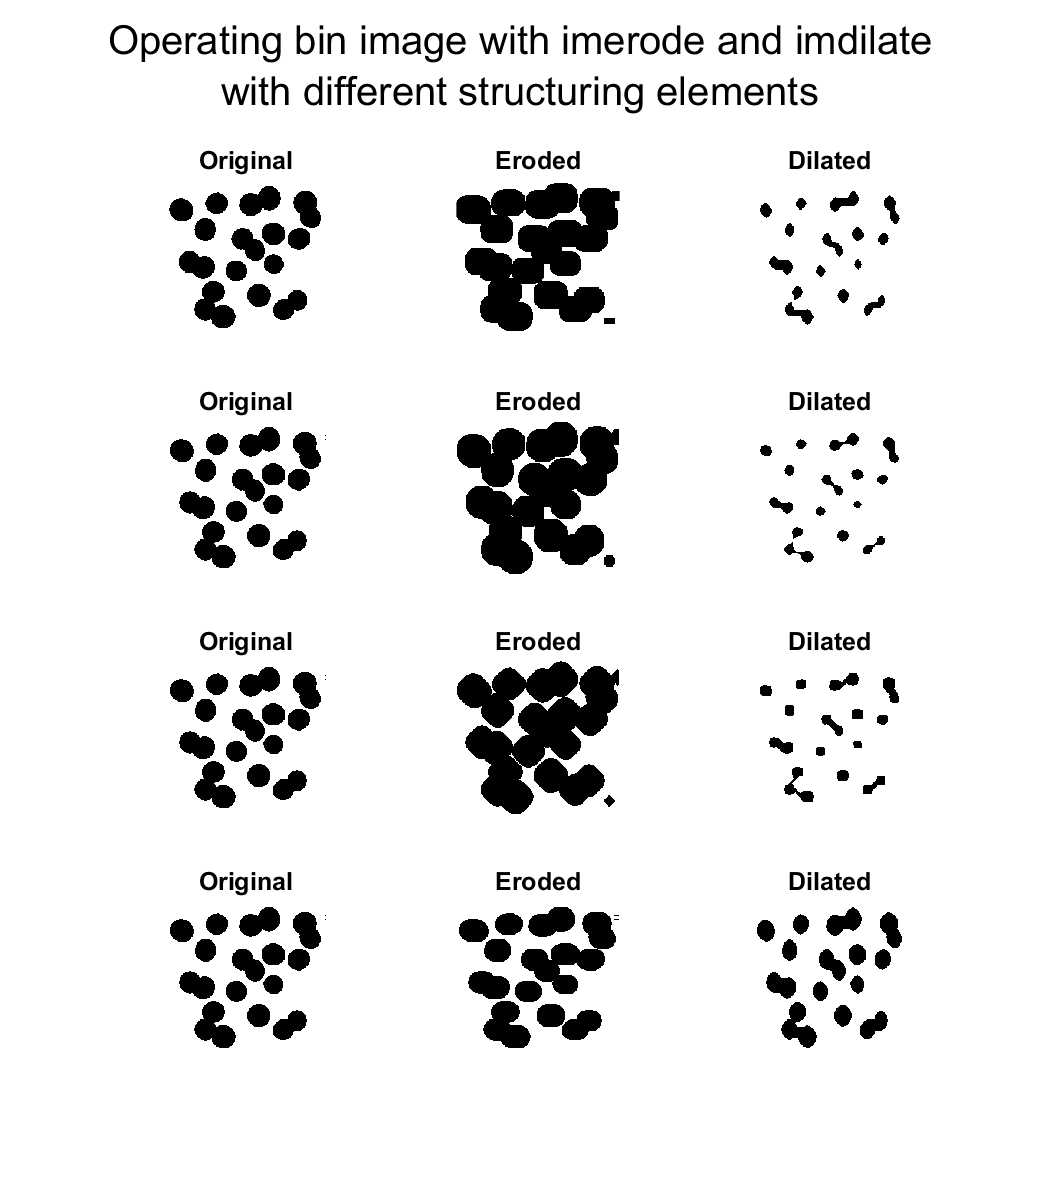
\includegraphics[width=0.8\linewidth]{Doc/Graphics/part2_Question2.png}
\end{figure}


\newpage
\textbf{Question 3} \textit{Extract internal and external edges of a binary image, and the morphological gradian.}
\begin{figure}[h]
    \centering
    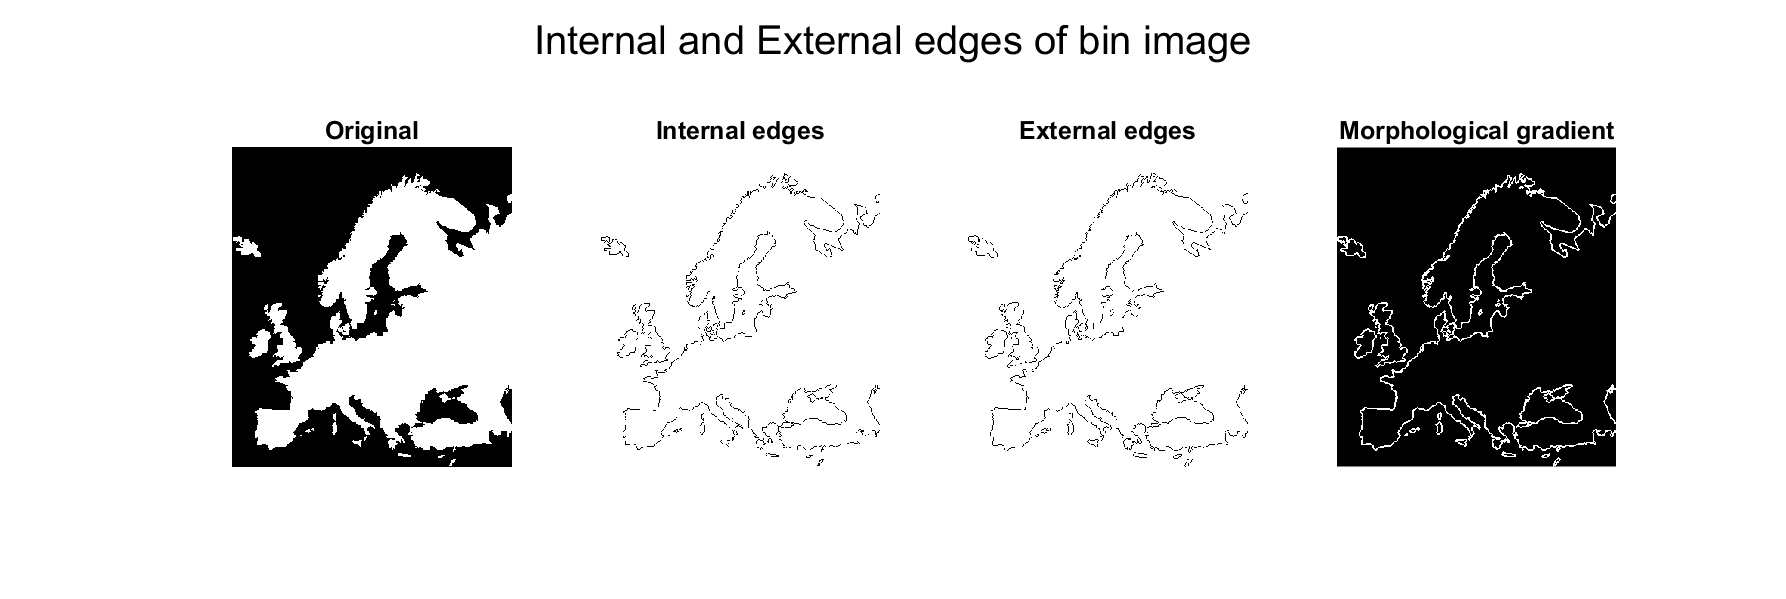
\includegraphics[width=1\linewidth]{Doc/Graphics/Part2_Question3.png}
\end{figure}


\textbf{Question 4} \textit{As an exercise, write an algorithm that show, in the map of Europe, the distance of each pixel w.r.t. the sea.}
\begin{figure}[h]
    \centering
    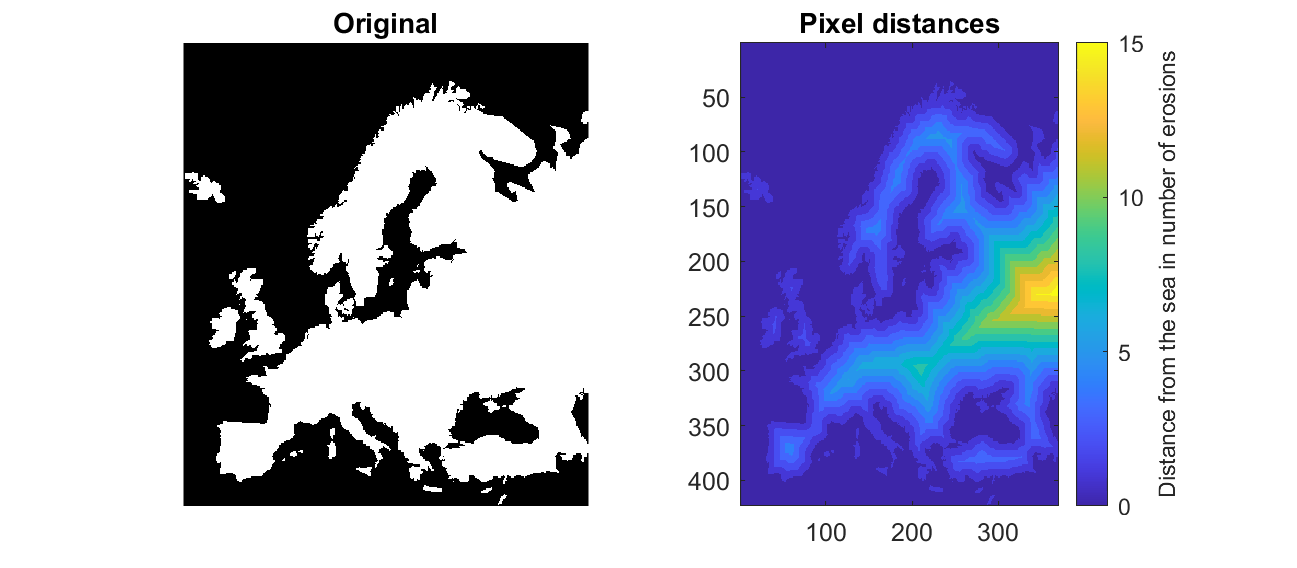
\includegraphics[width=0.75\linewidth]{Doc/Graphics/part2_Question4.png}
\end{figure}

\textbf{Question 5} \textit{Find an algorithm that detect rectangular objects of ’image2.jpg’.}

\textcolor{red}{TODO: Add pic from 5.}


\subsection{Morphological Filtering}
\subsubsection{Filters}
\textbf{Question 6} \textit{Define the two morphological filters called opening and closing. What are the effects on a binary image sur as ’image1.jpg’ (use the commands imopen and imclose)?}

\begin{itemize}
    \item \textbf{Opening filter:}
    some text

    \item  \textbf{Closing filter:}
    some text
\end{itemize}

\textcolor{red}{TODO: Add pic from 6}


\subsubsection{Form Detection}
\textbf{Question 7} \textit{The objective being to recognize some forms on images, find a simple algorithm to operate form detection}

See Question 5.


\textbf{Question 8} \textit{Apply a salt-and-pepper noise: what’s happen with your previous algorithm?}

The algorithm breaks and does not function at all due to the noise in the picture. See below:

\textcolor{red}{TODO add pic}

\subsubsection{Denoising}
\textbf{Question 9} \textit{Use the image Nebuleuse.jpg and apply a salt-and-pepper noise. De-noise the image by filtering.}

\textcolor{red}{TODO add pic}


\textbf{Question 10} \textit{Apply the same process to the ’Spain Beach’ image to isolate the beach itself.}

\textcolor{red}{TODO add pic}


\subsubsection{Top-Hat \& Black-Hat Filters}
\textbf{Question 11} \textit{Define op-hat and black-hat process in a 1D function: what is the associated process?}

\textcolor{red}{TODO Write shit here}


\textbf{Question 12} \textit{Define and operate top-hat and black-hat on a greyscale image. What do you observe?}

\textcolor{red}{TODO Write shit here}


\subsection{Morphological Skeletonization \& Segmentation}
\subsubsection{Skeletonization Process}
\textbf{Question 13} \textit{Write and operate a Skeletonization on the diplodocus.}
\textcolor{red}{TODO add pic}


\textbf{Question 14} \textit{Based on skelittization, find an algorithm that operate a segmentation in a binary image. Apply on ’image1.jpg’.}


\subsubsection{Image Segmentation}
\textbf{Question 15} \textit{Find a Skeletonization algorithm and operate on the Blood Cells image.}




\section{Shape Detection}
\label{sec:shape_detection}

Assignments for \textit{BE3\_ShapeDetection} practical.
\section{Introduction to Data Analysis: Data Classification}
\label{sec:data_analysis}

\subsection{Supervised Classification}
\textcolor{blue}{\textbf{Question 1:}}
\textit{Enumerate main supervized classification techniques and describe them in few lines.}

%~~~~~~~~~~~~~~ANSWER~~~~~~~~~~~~~~
Supervised Classification is... ???

Some typical Supervised Classification techniques are listed and described below:
\begin{enumerate}
    \item \textbf{k-Nearest Neighbours (k-NN):} The most simple classification algorithm where the principle is to find the \textit{k} closest data in the dataset to determine its class. 
    First a distance has to be defined, which is not always easy.

    
    \item \textbf{Maximum Likelihood:} A simple classifier based on the probability distribution.
    It assumes the data follows a known probability distribution (typically normal or Gaussian distr.) for each class.
    ML estimates the probability that a given data point belongs to each possible class and assigns it to the class with the highest likelihood.

    \begin{equation*}
        C^* = \underset{C_i}{\operatorname{argmax}} \, P(C_i \mid o)
    \end{equation*}

    
    \item Bayesian Classification:
    Based on the bayesian rule where given an observation \textit{o}, the \textit{prior} (a priori probability), is described as:
    \begin{equation*}
        P(C_i \mid o) = \frac{P(o \mid C_i) P(C_i)}{P(o)}
    \end{equation*}
    where $P(C_i \mid o)$ is called \textit{posterior} (a posterior probability).

    More text??

    
    \item \textbf{Linear Classification:}
    The most simple classification rule, where the objective is to establish a hyperplane, \textit{HP}, that separates the data into two groups:
    \begin{equation*}
    \begin{split}
        &\mathcal{H} : w_0 + \vec{w} \cdot \vec{x} = 0 \\
        &\text{In a \textit{n}-D space:} \\
        &\mathcal{H} : w_0 + w_1 x_1 + w_2 x_2 + \cdots + w_n x_n = 0
    \end{split}
    \end{equation*}

    Linear Classification is only possible if the data is \textit{linearly separable}. If not, there are infinite solutions
    An example of Linear Classification is the Perceptron Algorithm, which bla bla
    
    
    \item Neural Networks:
    \item Decision Trees:
    \item Concept Lattices:
    \item Support Vector Machine
    \item Random Forests:
    \item etc.
\end{enumerate}



\textcolor{blue}{\textbf{Question 2:}}
\textit{Apply and compare the following algorithms:
\begin{enumerate}
    \item 1-NN (your programme)
    \item Neural Network
\end{enumerate}
on 'Spain Beach' image or another of your choice
}


\textcolor{blue}{\textbf{Question 3:}}
\textit{Search on internet one of the two the following algorithms and apply it to the same image
\begin{enumerate}
    \item SVM
    \item Ramdom Forest
\end{enumerate}
}




\subsection{Unsupervised Classification}
\textcolor{blue}{\textbf{Question 4:}}
\textit{Enumerate main unsupervized classification techniques and describe them in few lines.}


\textcolor{blue}{\textbf{Question 5:}}
\textit{Apply the following algorithms with the dedicated objective
\begin{enumerate}
    \item k-means algorithm to define the four classes automatically and speed-up the classification process
    \item Pseudo-Inverse technique to estimate the position of a planet
    \item PCA technique to reduce the size of an image
\end{enumerate}
}


% REFERENCES
\addcontentsline{toc}{section}{References}
\printbibliography

%\begin{appendices}
\section{Source Code}
\subsection{MATLAB code for \autoref{sec:introduction_to_computer_vision}}
\label{sec:appendix_a1}
\lstinputlisting[frame=single, language=MATLAB, numbers=left]{../src/part1.m}


\newpage
\subsection{MATLAB code for \autoref{sec:introduction_to_mathematical_morphology}}
\label{sec:appendix_a2}
\lstinputlisting[frame=single, language=MATLAB, numbers=left]{../src/part2.m}


\newpage
\subsection{MATLAB code for \autoref{sec:shape_detection}}
\label{sec:appendix_a3}
\lstinputlisting[frame=single, language=MATLAB, numbers=left]{../src/part3.m}


\newpage
\subsection{MATLAB code for \autoref{sec:data_analysis}}
\label{sec:appendix_a4}
\lstinputlisting[frame=single, language=MATLAB, numbers=left]{../src/part3.m}

\newpage
\addcontentsline{toc}{section}{B\, Assignment Sheets}
% Assignment sheets
\addcontentsline{toc}{subsection}{Assignment sheet for section 1}
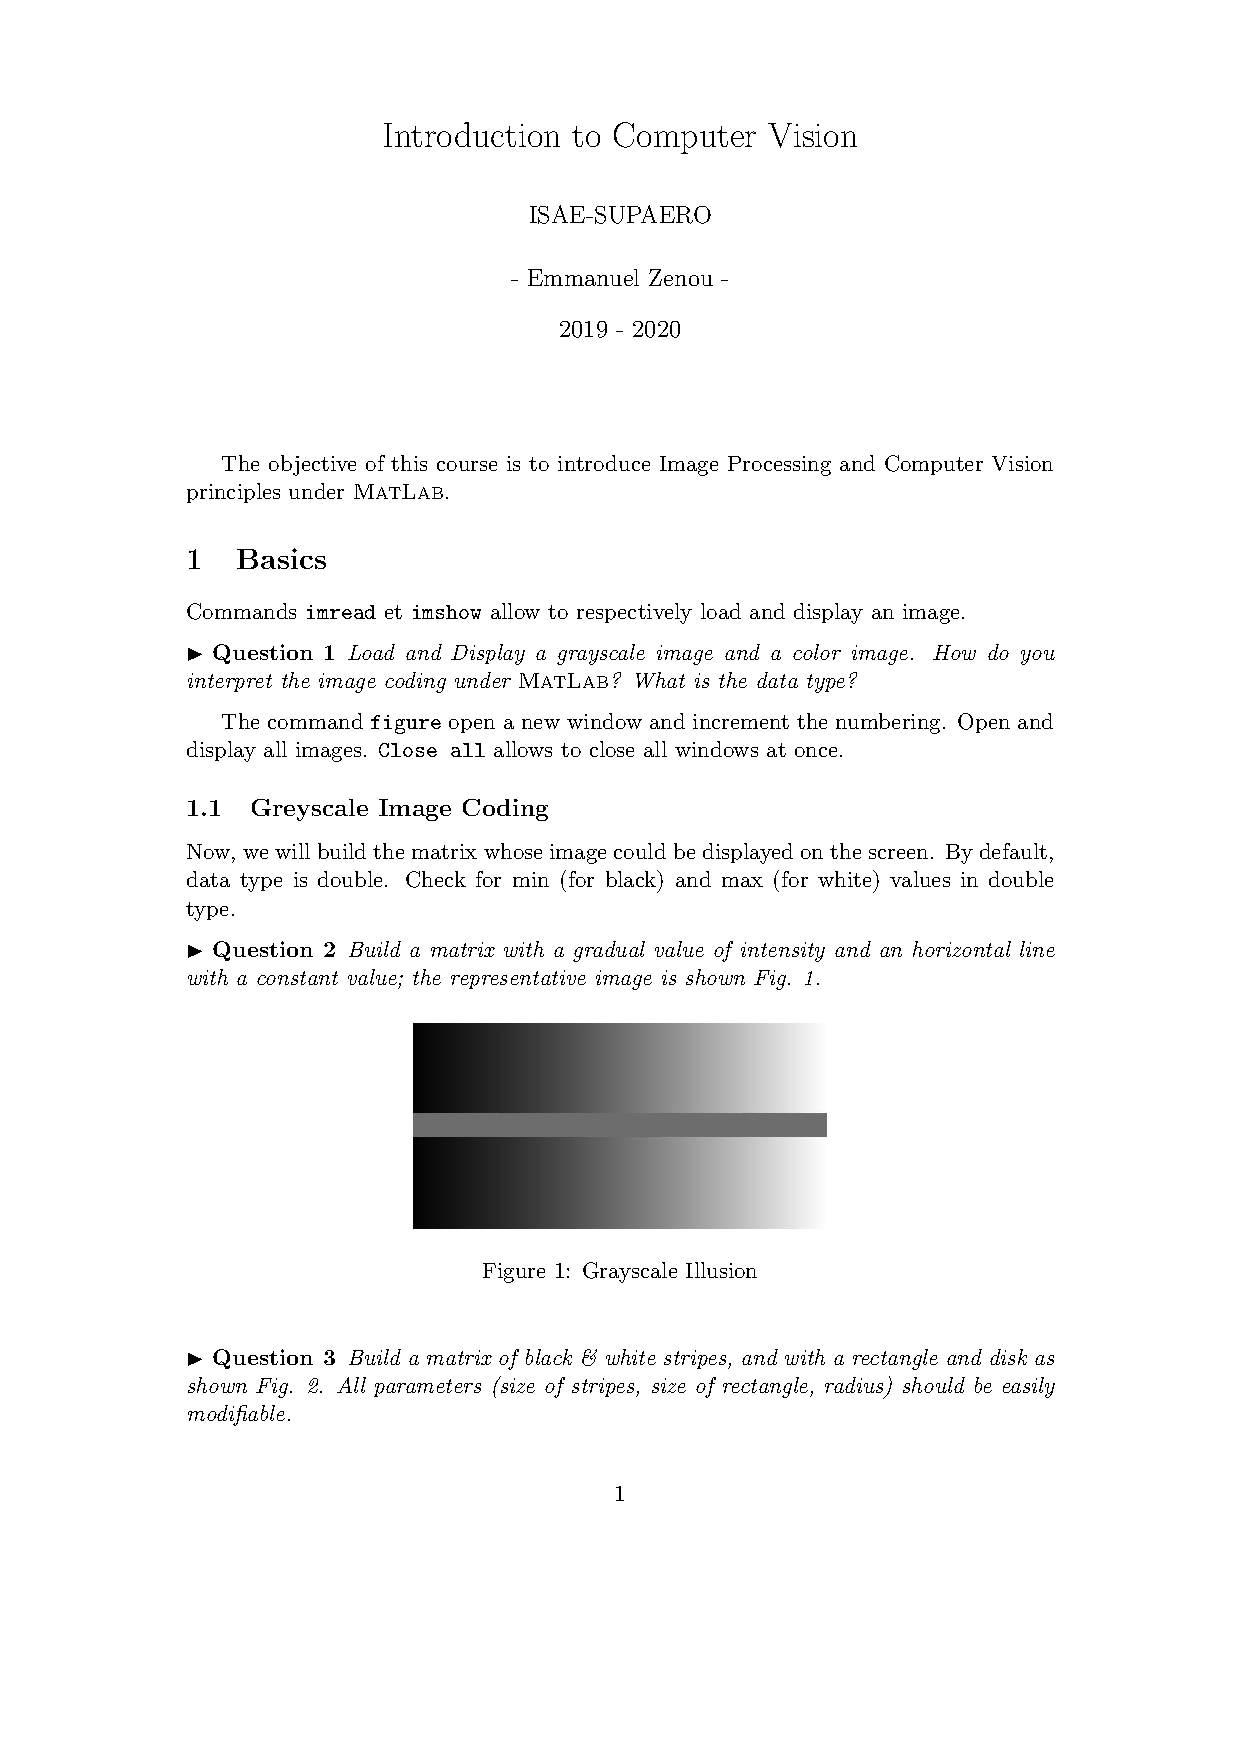
\includepdf[pages=-]{../BE1_IntroComputerVision/BE1_IntroComputerVision.pdf}

\addcontentsline{toc}{subsection}{Assignment sheet for section 2}
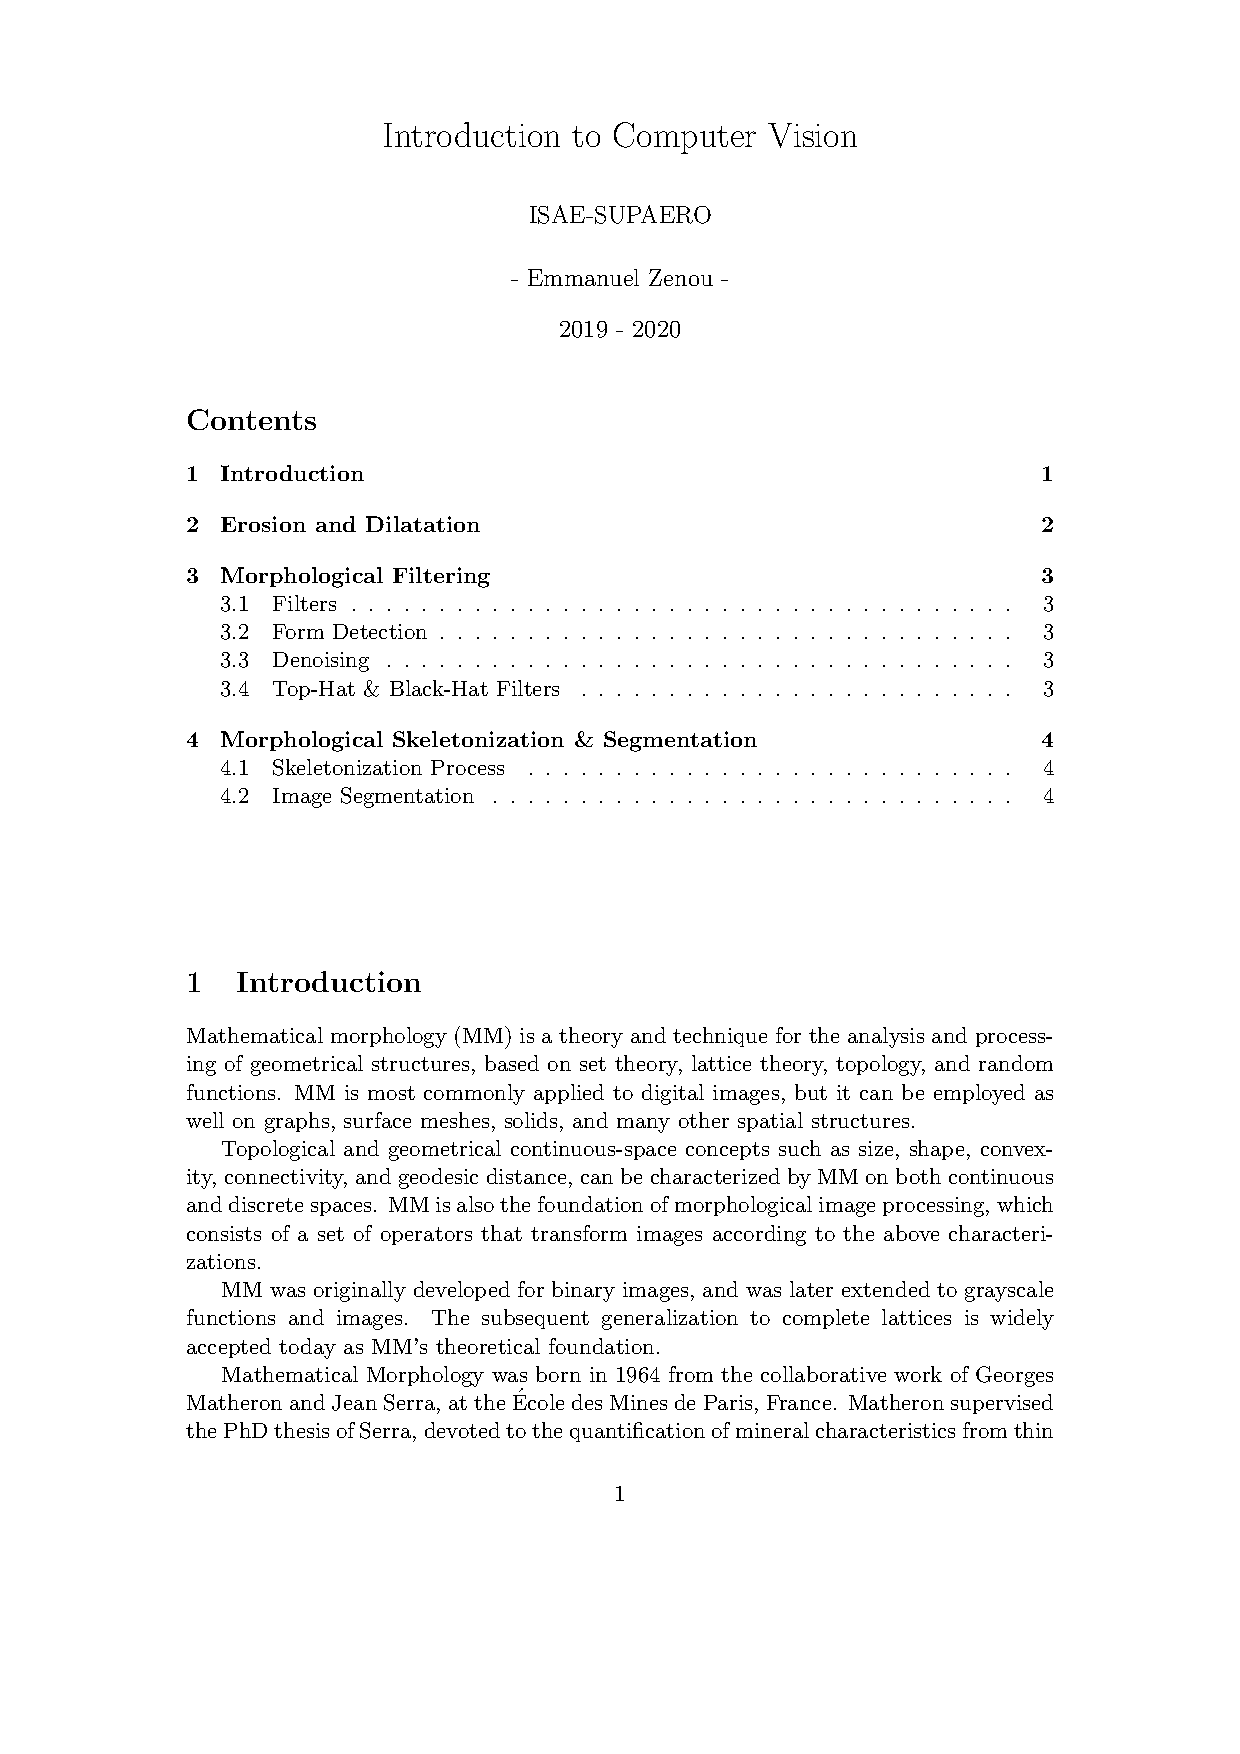
\includepdf[pages=-]{../BE2_IntroMorphoMath/BE2_IntroMorphoMath_en.pdf}

\addcontentsline{toc}{subsection}{Assignment sheet for section 3}
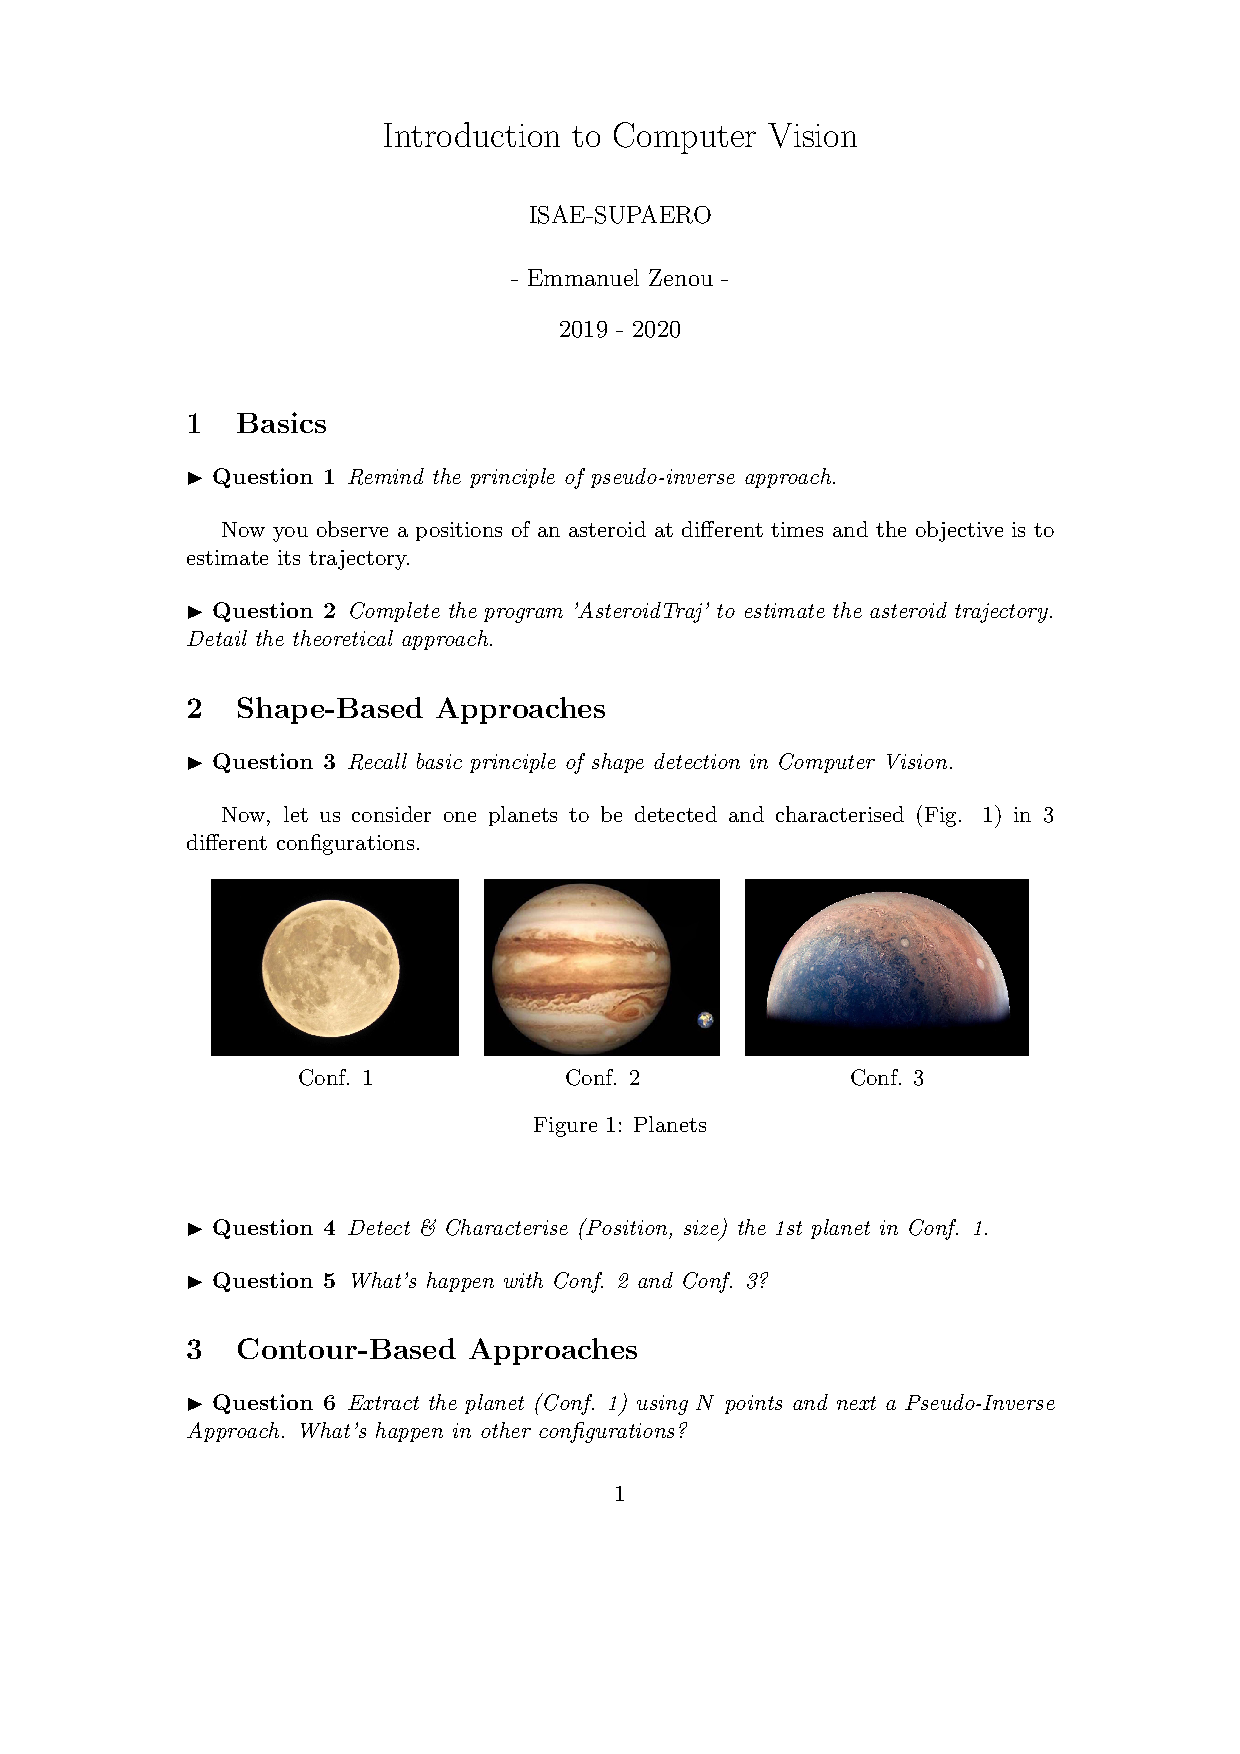
\includepdf[pages=-]{../BE3_ShapeDetection/BE3_ShapeDetection.pdf}

\addcontentsline{toc}{subsection}{Assignment sheet for section 4}

\includepdf[pages=-]{../Classif/PW_Classif.pdf}




\end{appendices}



\end{document}
